\subsection*{Дорожная библиотека -- индивидуальное задание}
\addcontentsline{toc}{subsection}{Дорожная библиотека -- индивидуальное задание}

\textbf{Задание:}\\
Построить и проанализировать дорожную имитационную модель над станцией метро Озерки.\\

\textbf{Решение:}\\
Имеется следующая схема надземной части станции метро Озерки. (Рисунок \ref{fig:road_plan})
\begin{figure}[h]
	\centering 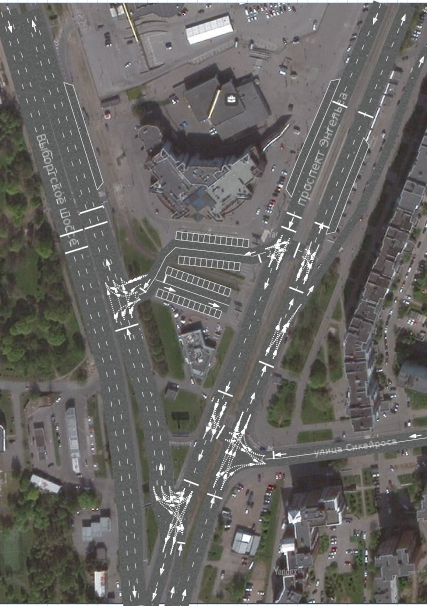
\includegraphics[scale=0.5]{road_plan}
	\caption{Надземная часть станции метро Озерки}
	\label{fig:road_plan}
\end{figure}

Всего существует три основных направления движения: проспект Энгельса (основная и встречная полосы), Выборгское шоссе (основная и встречная полосы), улица Сикейроса (основная и встречная полосы), так же имеется <<карман>> на встречной полосе проспекта Энгельса куда также могут отправляться машины.\\

На территории торгового центра имеется парковка где машины могут оставаться.\\

Машины, которые движутся по основному направлению проспекта Энгельса могут: заехать на парковку, повернуть на встречную полосу проспекта Энгельса, свернуть на улицу Сикейроса, повернуть на Выборгское шоссе или продолжить своё движение по текущему направлению.\\

Машины, которые движутся по встречному направлению проспекта Энгельса могут: повернуть на Выборгское шоссе, повернуть на улицу Сикейроса, повернуть на основную полосу проспекта Энгельса, свернуть в <<карман>> или продолжить своё движение по текущему направлению.\\

Машины, которые движутся по основному направлению улицы Сикейроса могут повернуть на встречную полосу проспекта Энгельса. Машины, которые движутся по встречному направлению улицы Сикейроса просто продолжают своё движение в данном направлении.\\

Машины, которые едут по основному направлению Выборгского шоссе просто продолжают своё движение в данном направлении. Машины, которые едут по встречному направлению Выборгского шоссе могут: заехать на парковку или продолжить своё движение по текущему маршруту.\\

Когда машина заезжает на парковку, то она может выбрать один из четырёх парковочных лотов. Когда у машины заканчивается её время пребывание на парковке, то она возвращается либо на основную линию проспекта Энгельса, либо на встречную линию Выборгского шоссе.\\

Также в данной модели предусмотрены светофоры и пешеходный переход, которые были скорректированы, на основе реальных данных.\\

Также можно встретить автобусы, которые двигаются по нескольким маршрутам:
\begin{itemize}[topsep=0pt,itemsep=-1ex,partopsep=1ex,parsep=1ex]
	\item проспект Энгельса (основное направление)
	\item проспект Энгельса (основное направление) $\rightarrow$ Выборгское шоссе (встречное направление)
	\item проспект Энгельса (встречное направление) $\rightarrow$ Выборгское шоссе (встречное направление)
	\item проспект Энгельса (встречное направление) $\rightarrow$ улица Сикейроса (встречное направление)
	\item проспект Энгельса (встречное направление)
	\item улица Сикейроса (основное направление) $\rightarrow$ проспект Энгельса (встречное направление)
\end{itemize}

Для данных маршрутов предусмотрены остановки, на которых останавливаются автобусы.

\newpage

В соответствии с описанием данная модель была реализована в среде моделирования \textit{AnyLogic} (Рисунок \ref{fig:road_anylogic_model}).

\begin{figure}[h]
	\centering 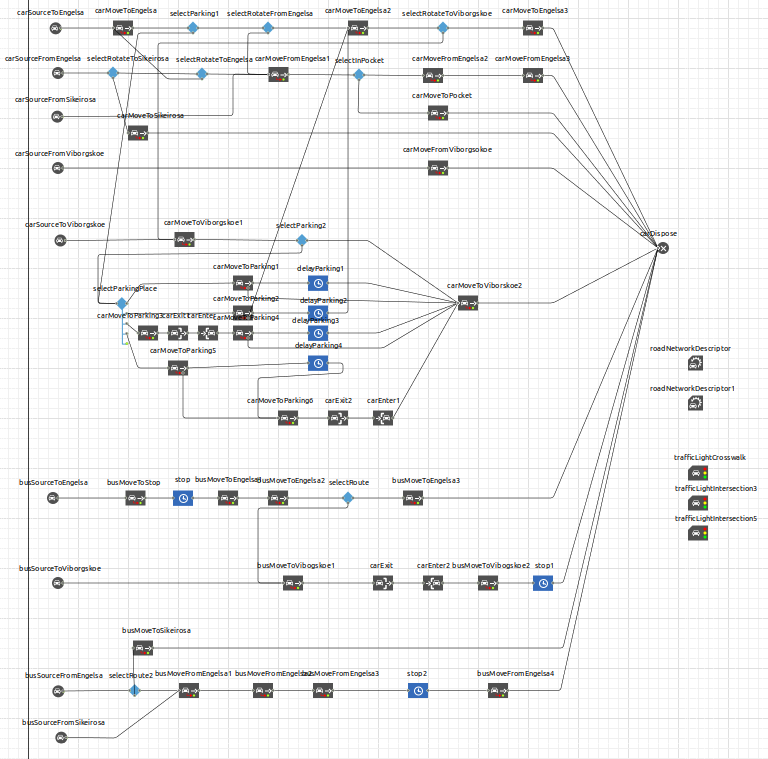
\includegraphics[scale=0.4]{road_anylogic_model}
	\caption{Модель в среде \textit{AnyLogic}}
	\label{fig:road_anylogic_model}
\end{figure}

Данная модель имеет статический потом интенсивности машин и автобусов.\\

\newpage

Также была построена визуализация модели (2D и 3D) и тепловая карта, которая соотвествует плотности различных участков дороги. (Рисунок \ref{fig:road_visualization})

\begin{figure}[h]
	\centering 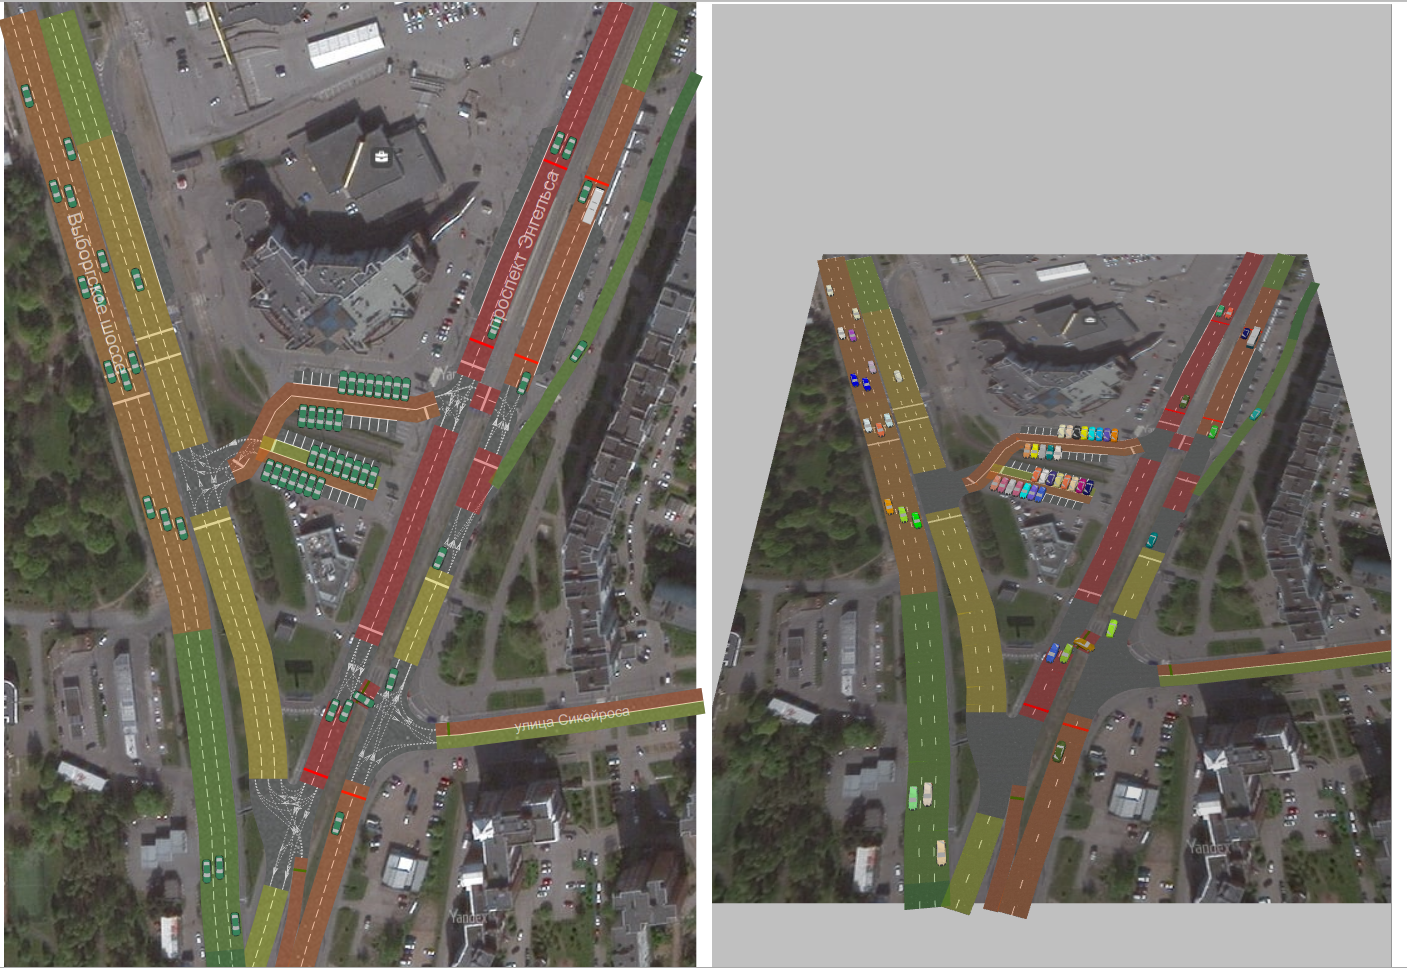
\includegraphics[scale=0.3]{road_visualization}
	\caption{Модель в среде \textit{AnyLogic}}
	\label{fig:road_visualization}
\end{figure}

На данной тепловой карте можно видеть, что из-за достаточно частых светофоров одним из самых плотных участков является основное направление проспекта Энгельса. Также из-за достаточно резкого поворота на встречном направлении проспекта Энгельса имеется плотный участок.